\begin{document}
	%TODO:  La puntuación log(UPSM) y el error de clasificación obtenido en todos los modelos para cada una de las tres clases de modelos.
	% TODO: El mejor modelo seleccionado de cada clase y su justificación de porque es el mejor. Mostrar también el dibujo de la red bayesiana para cada uno de estos tres modelos (incluso para el caso de la red bayesiana naive). Recordar que weka te permite visualizar la red bayesiana del modelo aprendido.
	En aquest apartat, es pot veure els valors, tant de la puntuació $\log(UPSM)$ com el percentatge d'error de la classificació, obtinguts en els diferents models de cadascuna de les classes de models. 
	\subsection{Models de la classe 1}
	\begin{enumerate}
		\item \textbf{log(UPSM):} -92608.96126554035 \textbf{Error de classificació:} 48.4167 \%
		\item \textbf{log(UPSM):} -92139.67866809308 \textbf{Error de classificació:} 48.4167 \%
		\item \textbf{log(UPSM):} -92388.27489566772 \textbf{Error de classificació:} 48.4167 \%
		\item \textbf{log(UPSM):} -92227.05224681877 \textbf{Error de classificació:} 48.4484 \%
		\item \textbf{log(UPSM):} -92066.4712487785 \textbf{Error de classificació:} 48.4167 \%
		\item \textbf{log(UPSM):} -92302.15263672064 \textbf{Error de classificació:} 48.4167 \%
		\item \textbf{log(UPSM):} -92180.71383973274 \textbf{Error de classificació:} 48.4167 \%
		\item \textbf{log(UPSM):} -92586.42609497187 \textbf{Error de classificació:} 48.4167 \%
		\item \textbf{log(UPSM):} -92245.67223271335 \textbf{Error de classificació:} 48.4167 \%
		\item \textbf{log(UPSM):} -93188.71009303001 \textbf{Error de classificació:} 48.4167 \%
	\end{enumerate}
	\vspace{0.5cm}
	Per a poder seleccionar el millor model dels anteriors, ens hem de fixar sobretot en quin d'ells ens classifica correctament un major nombre d'instàncies i, per tant, vaga la redundància, quin model té el menor percentatge d'error de classificació.\\
	\\
	Com es pot observar, tots els models tenen el mateix percentatge d'error excepte un, el qual es pot descartar directament, ja que és més alt que la resta. Entre els altres models, no es sorprenent que el percentatge no variï, ja que es pot observar en les dades tan inicials com després de separar-les en els conjunts d'aprenentatge i de prova,  la tendència d'un 50\% de casos en els quals el valor d'\verb|overall_satisfaction| és de 4.5.
	Això és a causa de dos factors principals:
	\begin{itemize}
		\item La seed, estipulada a l'hora de partir en dos el dataset, no genera una partició totalment desigual de l'altra. En altres paraules, el contingut de les dades en els dos datasets (tant en l'entrenament, com en l'evaluació) estan ben repartits, no segreguen casos únics i especials i gràcies a això no s'ha produït overfitting, ja que, en cas de tenir casos molt especials en l'avaluació, o en el training set, es tindria un error de classificació més alt.
		\item Més de 6000 casos del dataset total (contant entrenament i evaluació), el seu \texttt{overall\_satisfaction} és 4.5. Clarament, això afavorirà a la xarxa de bayesiana de predir 4.5 per sobre d'altres puntuacions. Si l'entrenament i el test fossin desiguals \footnote{La desigualtat es pot arribar a comprovar amb el coeficient de gini, per exemple.}, no es podria afirmar aquest raonament.
	\end{itemize}
Com que aquests factors no depenen en com està fet la xarxa en sí, sinó en el dataset, el resultat serà comú en els tres possibles tipus de xarxa bayesiana.
\\
\
	Per saber quin model és millor de l'actual classe, veient les dades proporcionades per Weka, s'arriba a la conclusió que els models es troben en una situació d'"empat". Una manera de resoldre'l, i la qual s'ha usat, és comparar els valors del $\log(UPSM)$ de cada model.
	\\
	\\
	Per concloure, es considera que, el millor model d'entre els que tenen el millor percentatge en aquesta classe, serà aquell que tingui un \textit{UPSM score} més elevat, és a dir, el model que el seu $\log(UPSM)$ sigui més alt\footnote{Com que els valors es troben en negatiu, el valor més gran és el que té el valor absolut més petit.}. Per tant, considerarem com a millor model de la classe 1, el classificat amb el nombre 5, del qual es pot observar la seva representació gràfica a la Figura \ref{fig:model1}.
	
	\begin{figure}[H]
		\centering
		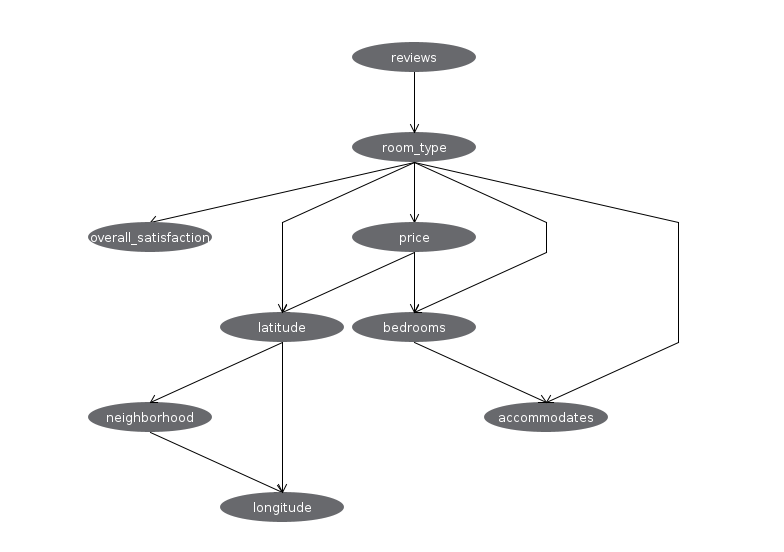
\includegraphics[width=12cm]{imgs/modelclasse1.png}
		\caption{Millor model de la classe 1}
		\label{fig:model1}
	\end{figure}
	\vspace{0.5cm}
	
	\subsection{Model de la classe 2}
	\begin{enumerate}
		\item \textbf{log(UPSM):} -117515.15847723951 \textbf{Error de classificació:} 48.4484 \%
	\end{enumerate}
	\vspace{0.5cm}
	En el cas de la segona classe, només hi trobem un model possible, per tant, serà aquest és el que es considera millor. El fet que només n'hi hagi un de possible és degut al fet que aquest model és el corresponent a la xarxa bayesiana \textit{naive}, tenint com a variable de classe \verb|overall_satisfaction|, el qual és un model únic.\\
	\\
	A la figura \ref{fig:model2} es pot veure la representació gràfica d'aquest model.
	\vspace{0.3cm}
	\begin{figure}[H]
		\centering
		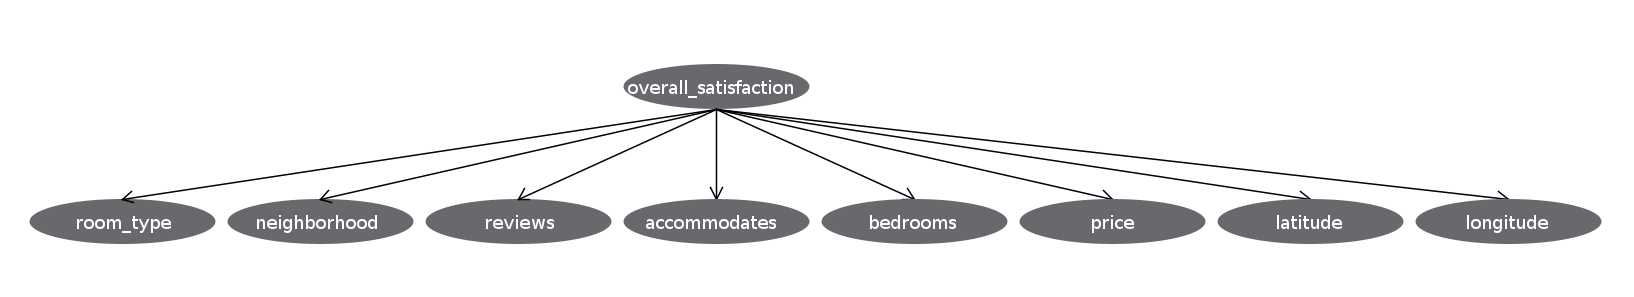
\includegraphics[width=15cm]{imgs/model2.png}
		\caption{Millor model de la classe 2}
		\label{fig:model2}
	\end{figure}
	\vspace{0.5cm}
	\subsection{Models de la classe 3}
	\begin{enumerate}
		\item \textbf{log(UPSM):} -96800.35169816265 \textbf{Error de classificació:} 48.3534 \%
		\item \textbf{log(UPSM):} -95829.88423245584 \textbf{Error de classificació:} 48.86 \%
		\item \textbf{log(UPSM):} -95565.62218051209 \textbf{Error de classificació:} 48.8284 \%
		\item \textbf{log(UPSM):} -95859.94046082163 \textbf{Error de classificació:} 48.4167 \%
		\item \textbf{log(UPSM):} -97231.01625115846 \textbf{Error de classificació:} 48.7334 \%
		\item \textbf{log(UPSM):} -96894.65682950999 \textbf{Error de classificació:} 48.3217 \%
		\item \textbf{log(UPSM):} -95822.6410503832 \textbf{Error de classificació:} 48.67 \%
		\item \textbf{log(UPSM):} -97094.31982431604 \textbf{Error de classificació:} 48.1951 \%
		\item \textbf{log(UPSM):} -95604.5241813889 \textbf{Error de classificació:} 48.575 \%
		\item \textbf{log(UPSM):} -96108.4925816474 \textbf{Error de classificació:} 48.3534 \%
	\end{enumerate}
	\vspace{0.5cm}
	Per tal de poder escollir el millor model d'aquesta classe, s'ha fet de la mateixa manera que en la classe 1. Tot i això, en aquest cas sí que s'ha pogut veure més diversitat de percentatges d'error en els diferents models. Per aquest motiu, no ha estat necessari comparar els valors de l' \textit{UPSM}.\\
	\\
	Els percentatges són bastant semblants entre si, ja que el fet d'encertar algunes variables més que un altre model, no implica un gran canvi en el percentatge d'encerts, a causa de la gran quantitat d'instàncies que tenim en el test. Malgrat tot, hi ha un model que ha encertat algunes instàncies més que la resta. Per tant, considerem com a millor model de la classe 3, classificat amb el nombre 8, del qual es pot observar la seva representació gràfica a la Figura \ref{fig:model3}.
	\begin{figure}[H]
		\centering
		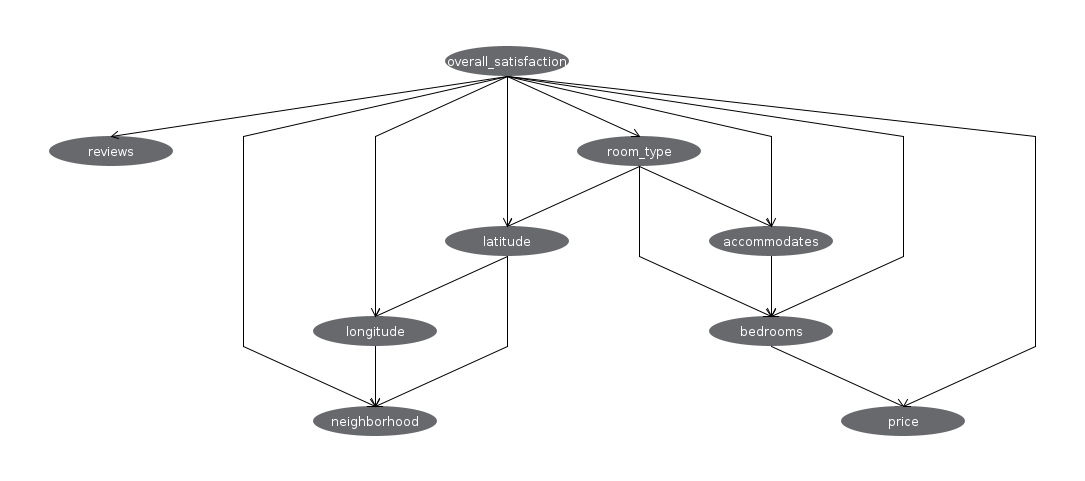
\includegraphics[width=15cm]{imgs/modelclasse3.png}
		\caption{Millor model de la classe 3}
		\label{fig:model3}
	\end{figure}
\end{document}